\documentclass{article}
\usepackage{tikz}
\usetikzlibrary{shapes, arrows.meta, positioning}
\begin{document}
\begin{figure}[ht]
\centering
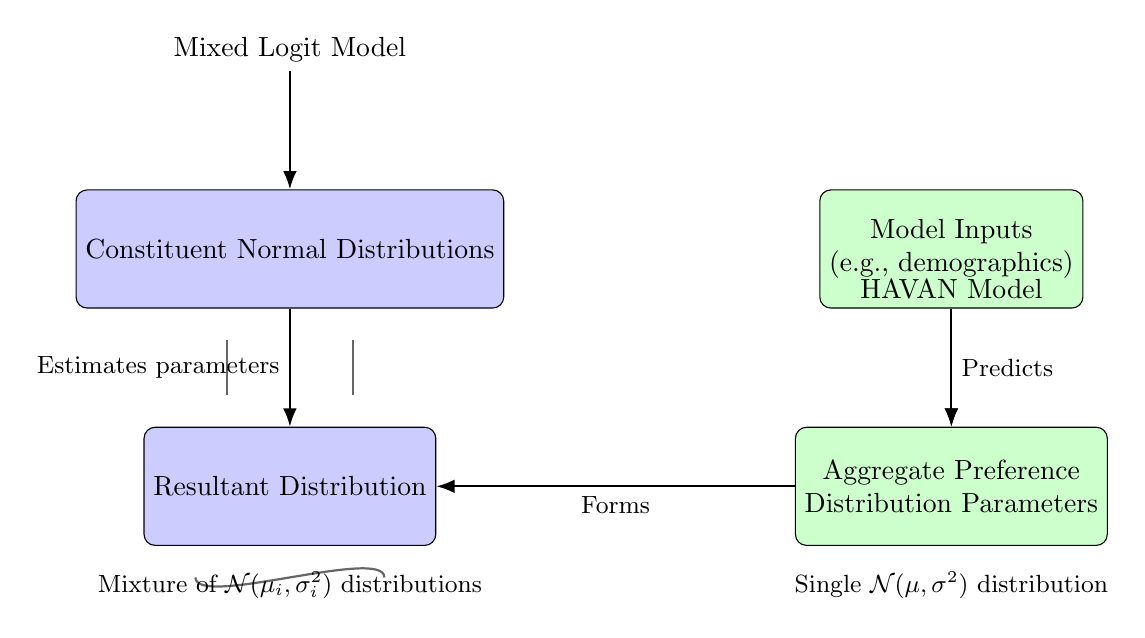
\begin{tikzpicture}[
    node distance = 1.5cm,
    process/.style = {rectangle, rounded corners, draw, fill=blue!20,
                      minimum width=3cm, minimum height=1.5cm, align=center},
    havan/.style = {rectangle, rounded corners, draw, fill=green!20,
                    minimum width=3cm, minimum height=1.5cm, align=center},
    arrow/.style = {-Latex, thick},
    dist/.style = {draw, thick, color=black!60}
]
% Mixed Logit Section
\node (constituent) [process] {Constituent Normal Distributions};
\node (resultant) [process, below=of constituent] {Resultant Distribution};
\node (mixed) [above=of constituent] {Mixed Logit Model};
% HAVAN Section
\node (inputs) [havan, right=4cm of constituent] {Model Inputs\\(e.g., demographics)};
\node (aggregate) [havan, below=of inputs] {Aggregate Preference\\Distribution Parameters};
\node (havan) [above=of aggregate] {HAVAN Model};
% Constituent Distributions (Visual Elements)
\foreach \x in {-0.8,0,0.8} {
    \draw[dist] ([shift={(\x, -0.4)}]constituent.south) 
        .. controls +(0,-0.3) and +(0,0.3) .. ([shift={(\x, -1.1)}]constituent.south);
}
% Resultant Distribution (Visual Element)
\draw[dist] ([shift={(-1.2, -0.4)}]resultant.south) 
    .. controls +(0,-0.4) and +(0,0.4) .. ([shift={(1.2, -0.4)}]resultant.south);
% Arrows and Labels
\draw[arrow] (constituent) -- node[left] {\small Estimates parameters} (resultant);
\draw[arrow] (inputs) -- node[right] {\small Predicts} (aggregate);
\draw[arrow] (aggregate) -- node[below] {\small Forms} (resultant);
\draw[arrow] (mixed) -- (constituent);
\draw[arrow] (havan) -- (aggregate);
% Annotations
\node[below=0.2cm of resultant, align=center, font=\small] 
    {Mixture of $\mathcal{N}(\mu_i, \sigma_i^2)$ distributions};
\node[below=0.2cm of aggregate, align=center, font=\small] 
    {Single $\mathcal{N}(\mu, \sigma^2)$ distribution};
\end{tikzpicture}
\caption{Comparison of preference distribution modeling approaches. 
The Mixed Logit model estimates parameters for individual constituent 
Normal distributions which combine to form the resultant distribution. 
The HAVAN model directly predicts parameters for an aggregate Normal 
distribution based on input variables.}
\end{figure}
\end{document}